\Transcb{yellow}{blue}{Hunting for Cosmic Neutrino sources}
\twocolumn
\begin{center}
\colorbox{yellow}{Neutrino production mechanism}\\
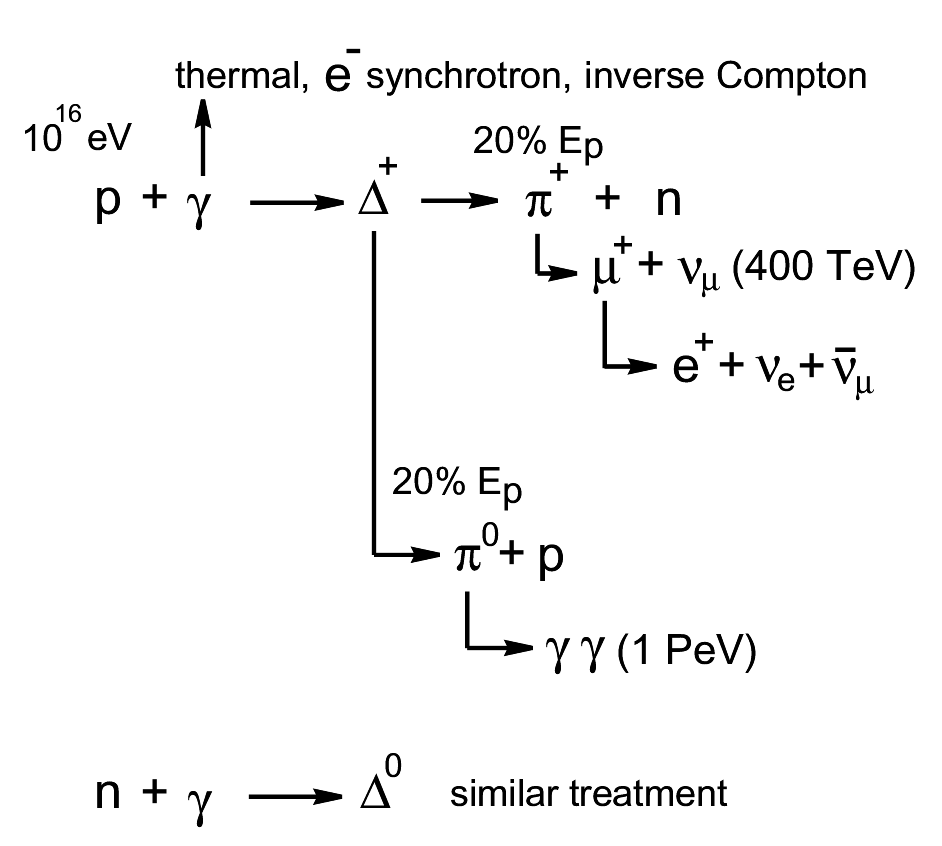
\includegraphics[keepaspectratio,width=13cm]{grb-engine2}
\end{center}
%
\begin{itemize}
\item $\Delta$ prod. threshold~: $E_{\gamma} \ge 10$ eV\\
      (UV photons)
\end{itemize}

\newpage
%
\begin{itemize}
\item Waxmann-Bahcall model
\item[] High-E $p$ diffuse out of the shocks
\item[] Observed CR $\rightarrow$ lower limit on $p$ flux 
\item[] {\blue Fraction of $p$ used for $\nu$ production ?}
\item Magn. confinement (Rachen, Ahlers)
\item[] Protons trapped, neutrons escape
\item[] CR observations provide the $n$ flux 
\item[] {\blue Direct relation CR $\leftrightarrow \nu$ flux}
\item Non-Cosmic Ray (Guetta, H\"{u}mmer)
\item[] Fixed fraction of $E_{\gamma}$ outflow as $p$
\item[] Protons not necessarily escape
\item[] {\blue Normalisation of proton fraction ?}
\item[] {\blue Fraction of $p$ used for $\nu$ production ?}
\item[$\ast$] \colorbox{yellow}{Let's search for high-E $\nu$ sources}
\end{itemize}

\Tr
\onecolumn
\begin{center}
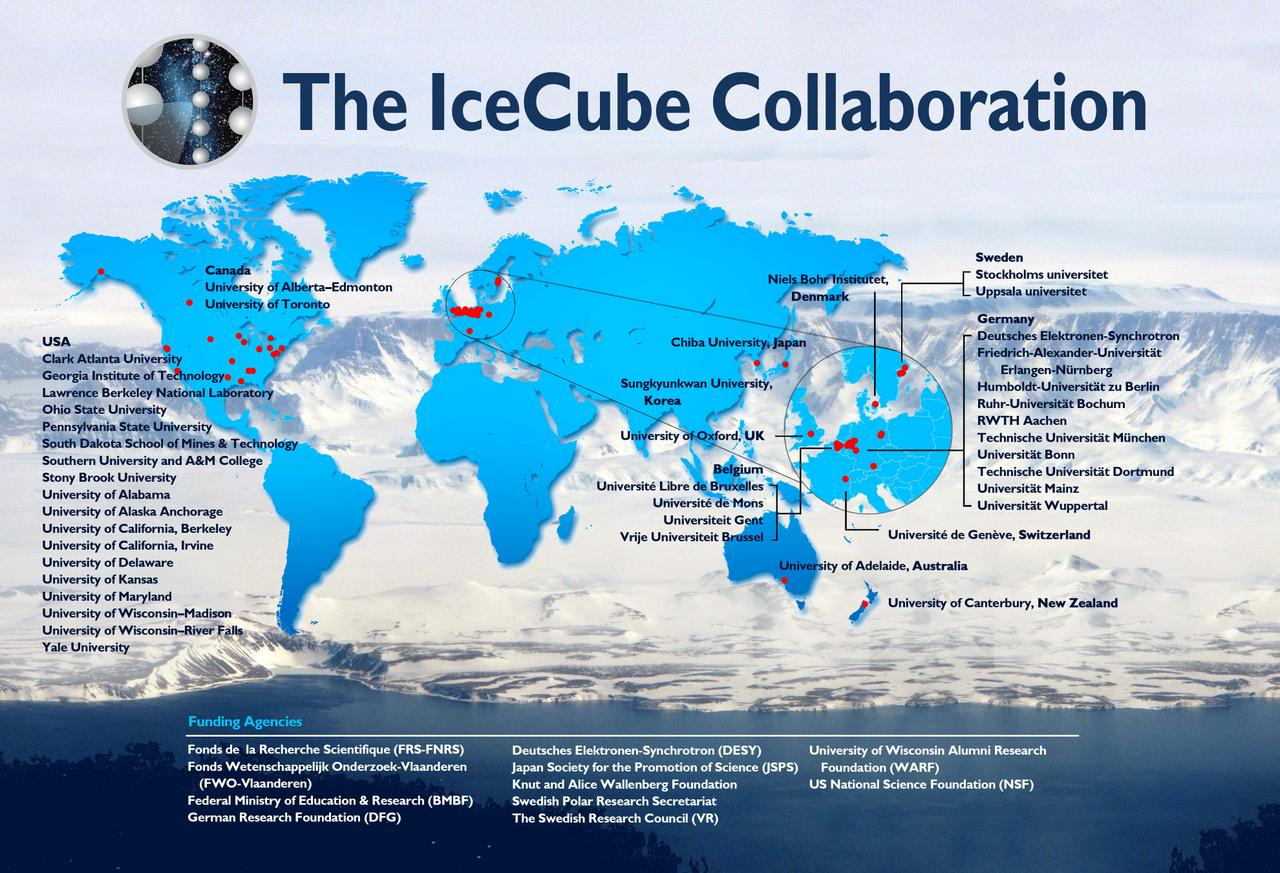
\includegraphics[keepaspectratio,height=15cm]{icecube-collab}
\end{center}

\Tr
\onecolumn
\begin{center}
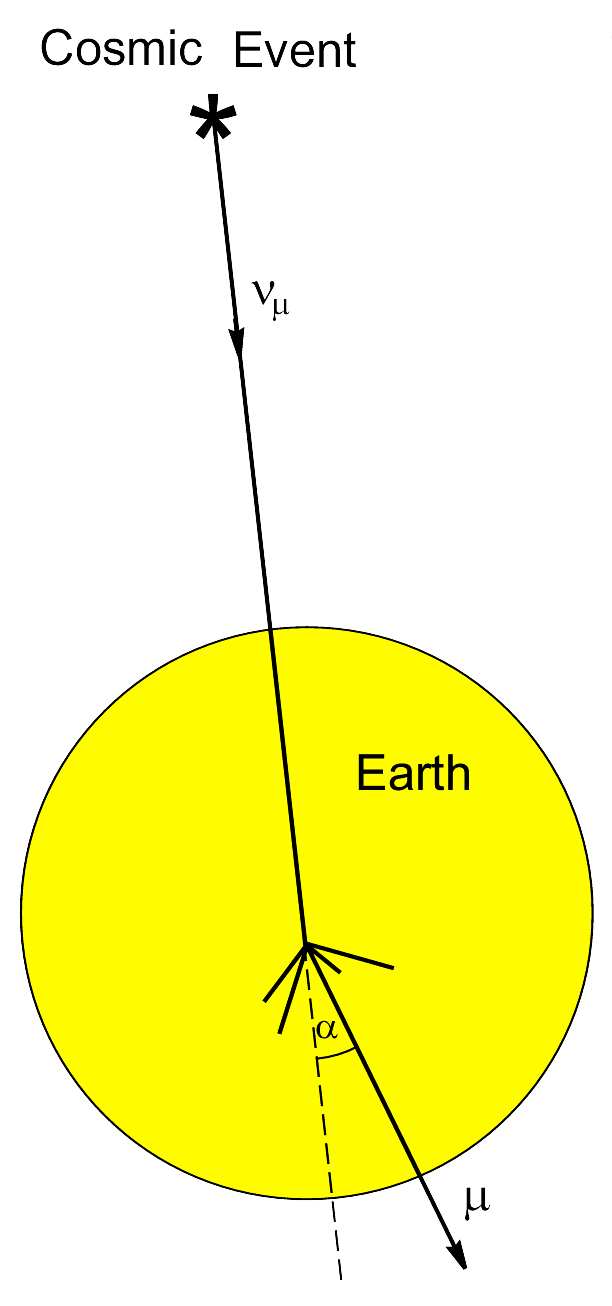
\includegraphics[keepaspectratio,height=14cm]{earth-shield} $\quad$
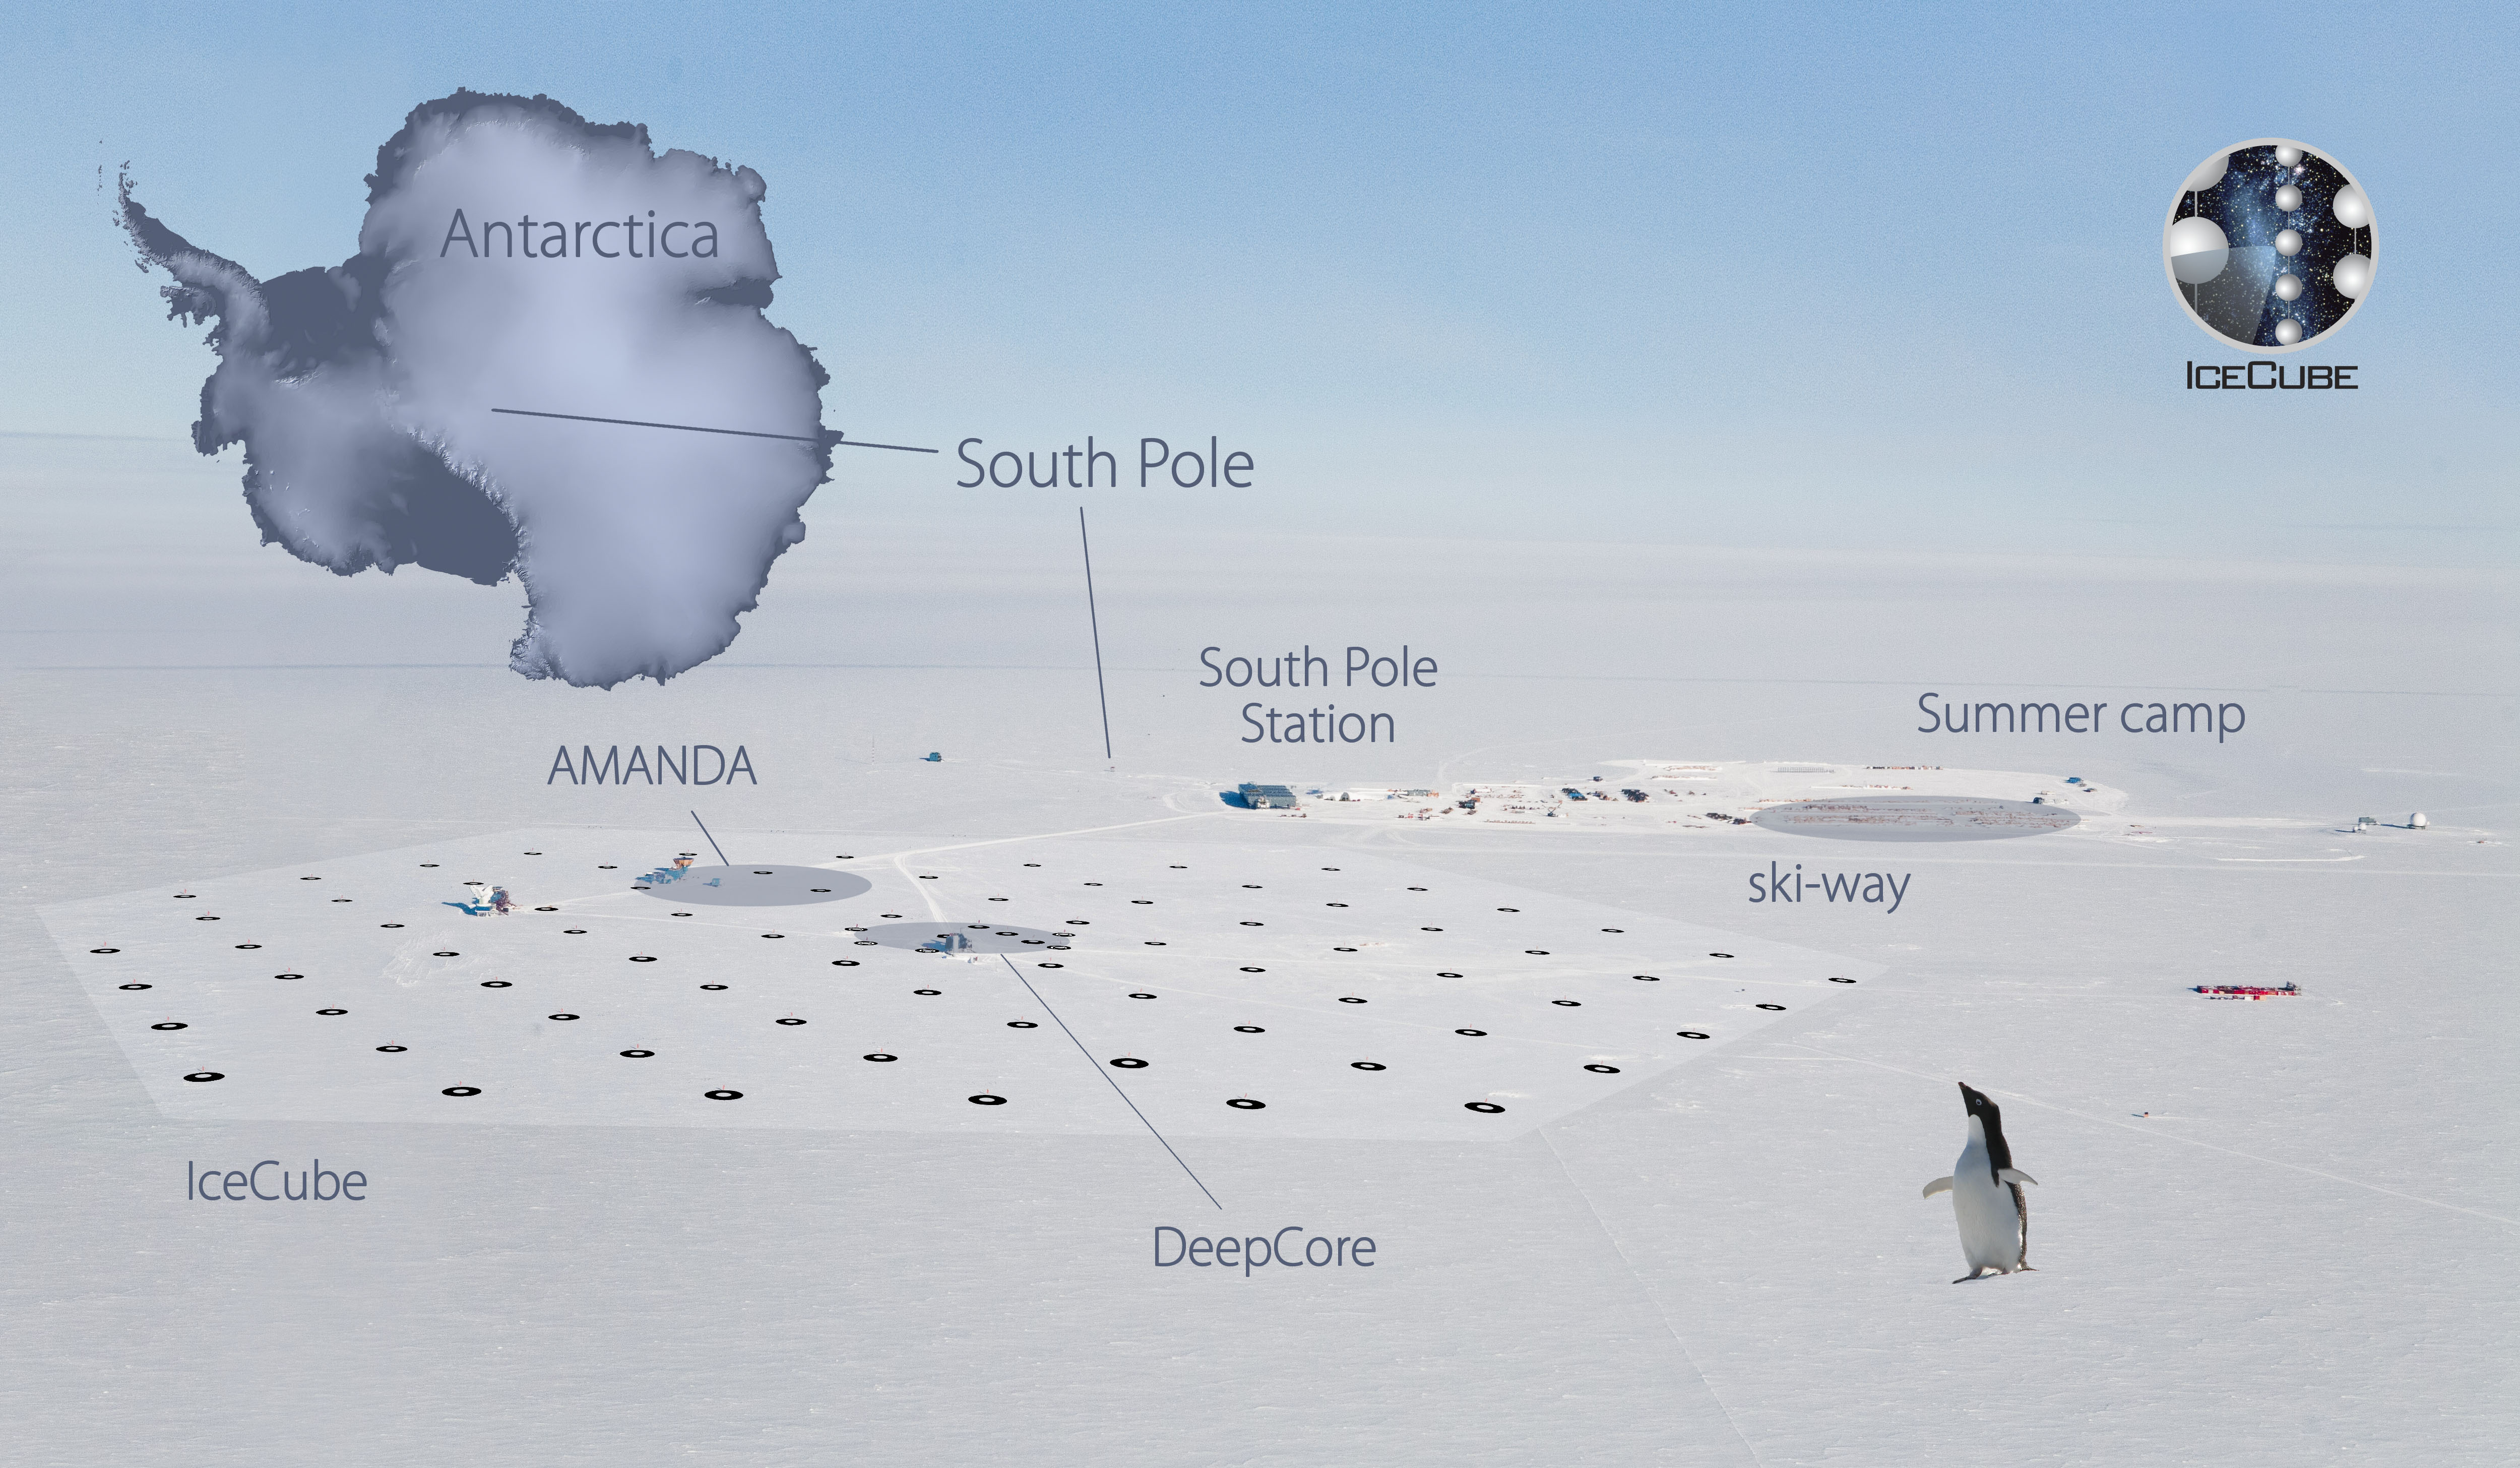
\includegraphics[keepaspectratio,width=18cm]{pole-view}
\end{center}

\Tr
\onecolumn
\begin{center}
{\blue The IceCube neutrino observatory}\\[3mm] 
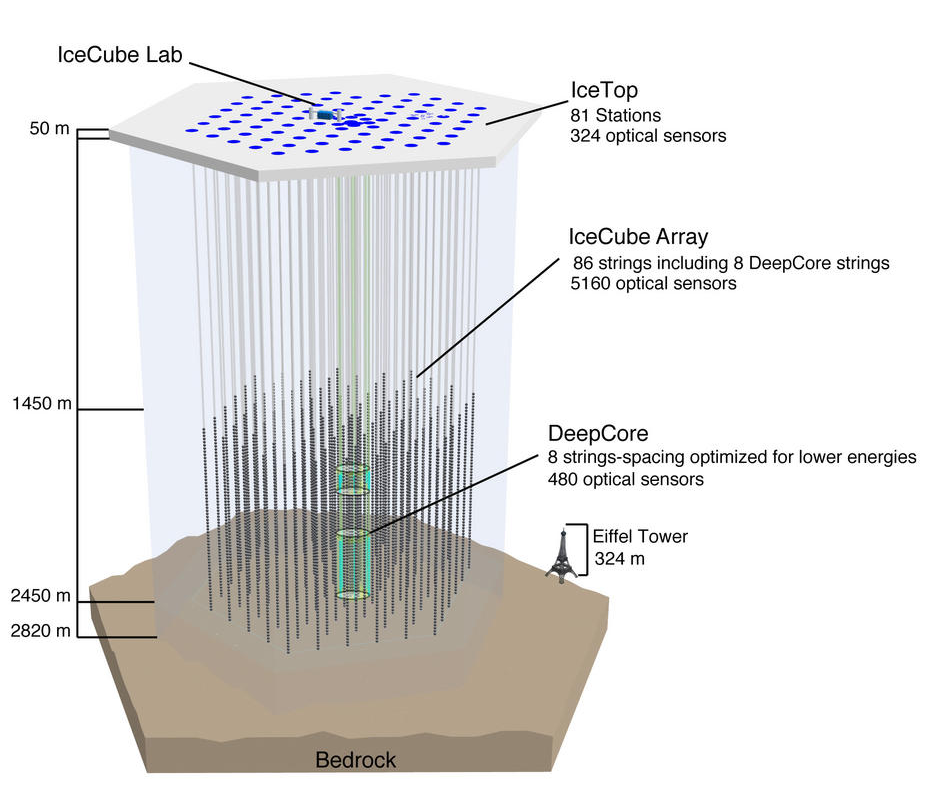
\includegraphics[keepaspectratio,height=14cm]{ic86-dc}
\end{center}

\Tr
\onecolumn
\begin{center}
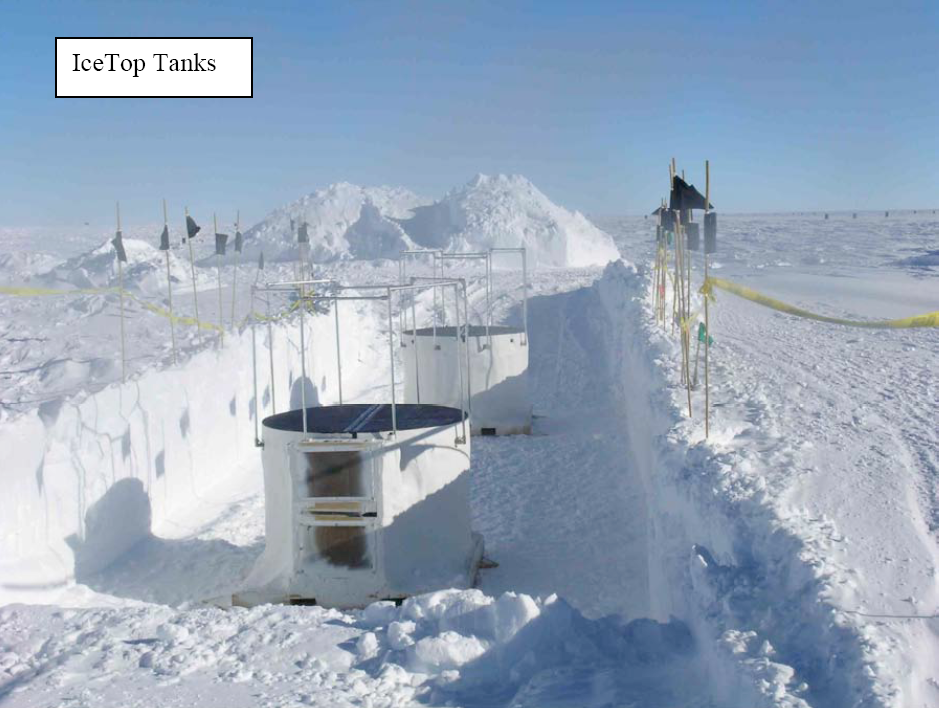
\includegraphics[keepaspectratio,height=14.5cm]{icetop-snow}
\end{center}

\Tr
\onecolumn
\begin{center}
{\blue The IceTop detection principle}\\[5mm] 
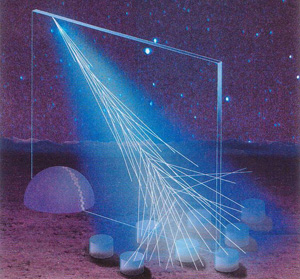
\includegraphics[keepaspectratio,height=14cm]{cr-shower}
\end{center}

\Tr
\onecolumn
\begin{center}
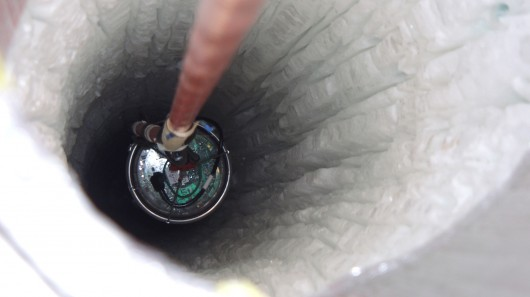
\includegraphics[keepaspectratio,height=14cm]{hole2}
\end{center}

\Tr
\twocolumn[\begin{center}{\blue The InIce detection principle}\end{center}]
\begin{center}
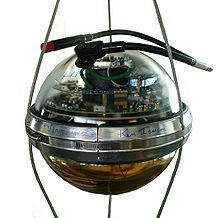
\includegraphics[keepaspectratio,height=6cm]{dom}\\[3mm]
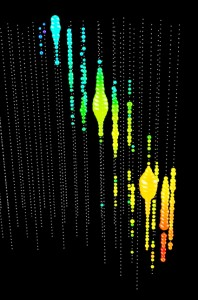
\includegraphics[keepaspectratio,height=7cm]{event}
\end{center}
%
\newpage
%
\begin{center}
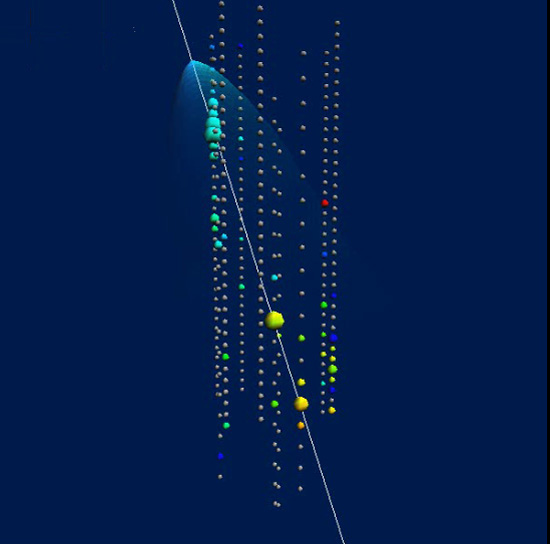
\includegraphics[keepaspectratio,width=13.5cm]{cone}
\end{center}

\Tr
\onecolumn
\begin{center}
{\red Muons from atmospheric interactions}\\[1cm]
{\blue The shadow of the Moon}\\[5mm]
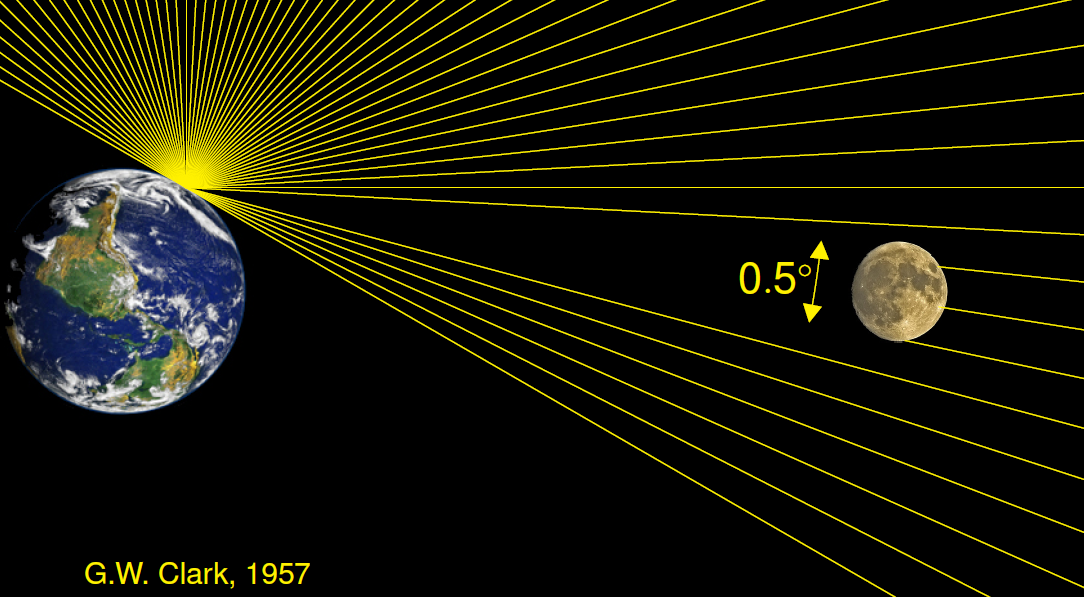
\includegraphics[keepaspectratio,height=8cm]{moon-shadow1}
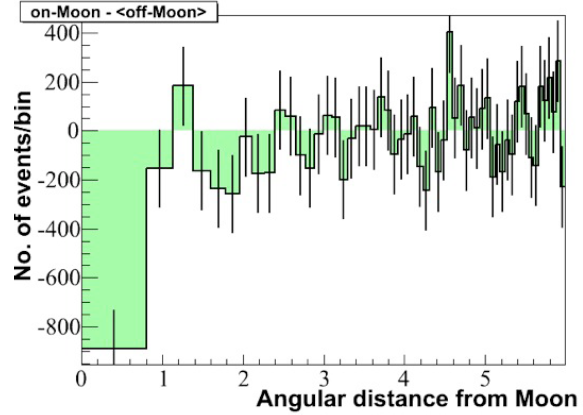
\includegraphics[keepaspectratio,height=8cm]{moon-shadow2}\\[1cm]
{\blue Angular resolution : $\sim 0.8^{\circ}$}
\end{center}

\Tr
\begin{center}
{\red Muons from atmospheric interactions}\\[1cm]
{\blue Cosmic ray anisotropy}\\[5mm]
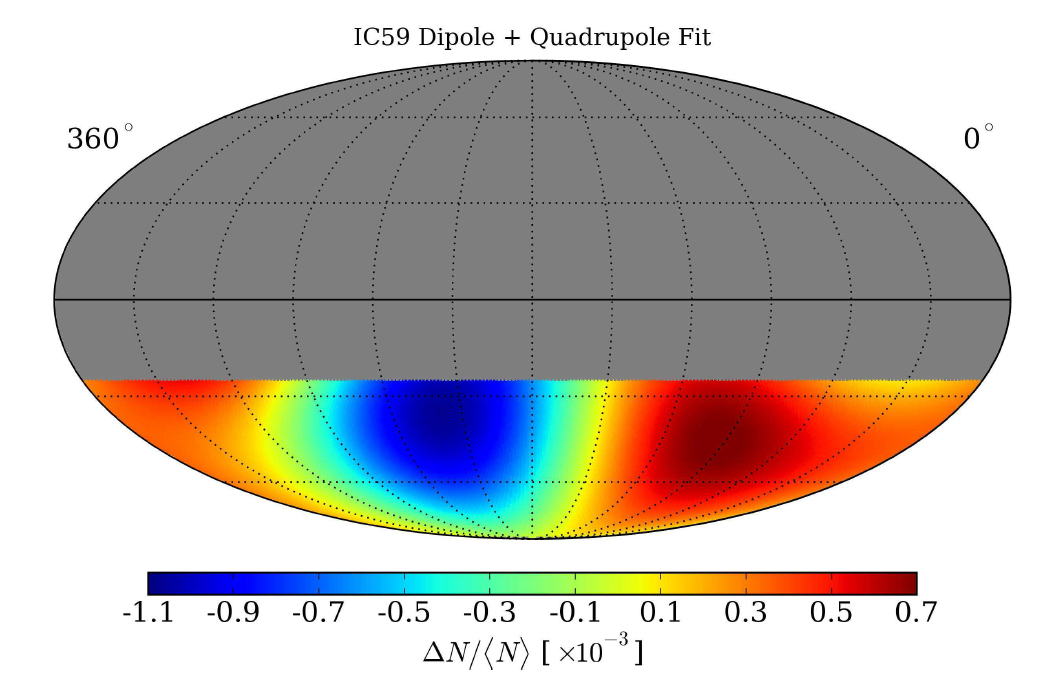
\includegraphics[keepaspectratio,height=12cm]{cr-anisotropy}
\end{center}

\Tr
\onecolumn
\begin{center}
{\blue IceCube neutrino equatorial skymap (ApJ 779 (2013) 132)}\\
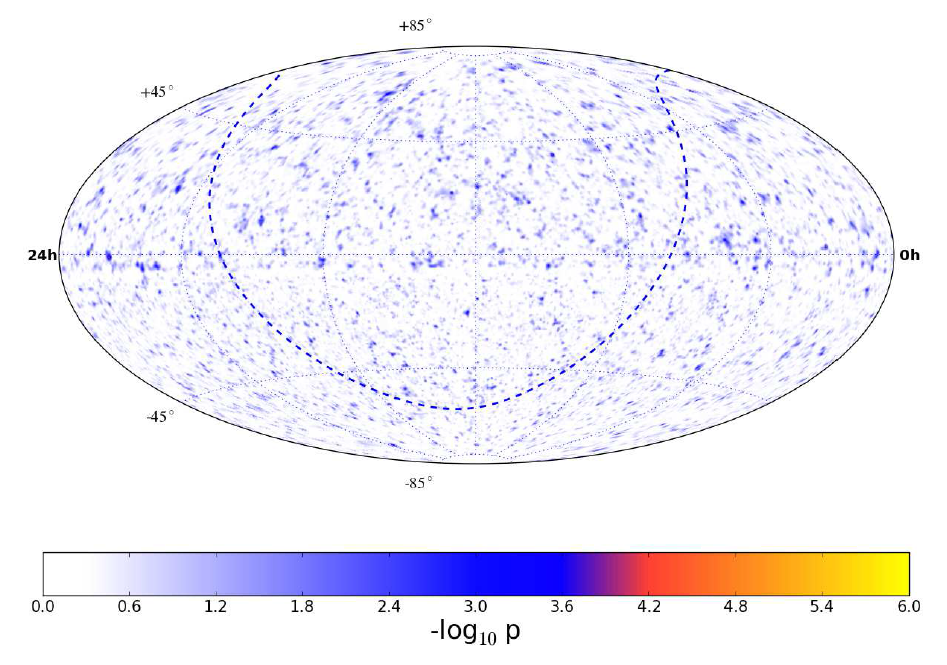
\includegraphics[keepaspectratio,height=12.5cm]{ic79+59+40-skymap}
\end{center}
Most significant excess : $\alpha =$ 2h~17m~0s $\quad \delta = 2.75^{\circ} \quad \text{P-value} = 1.96 \cdot 10^{-5}$\\
Randomised $\alpha$ data sets $\rightarrow$ post-trial : P-value=0.57
